%%% fs-seim-experiments - Experiments

\label {fs-experiments}

In order to estimate the performance, we implemented a prototype based on the proposed approach. As a stream processing task, we apply the computation of inverted index for 1000 Wikipedia documents. The logical pipeline of this computation is shown in Figure ~\ref{inverted-index}. First map operation accepts Wikipedia documents and outputs pairs of words and corresponding positions. The next part of the pipeline accepts pairs of word and positions and computes updated posting list and the actual changelog. 

This stateful transformation is implemented in the form of groping and map operation with a cycle, as it was shown in the previous section. Regarding the physical deployment, the full logical graph is deployed on each computational unit or worker. Documents are randomly shuffled before the first map operation. Word positions are partitioned by word before grouping. The other links are implemented as simple chain calls.

\begin{figure}[htbp]
  \centering
  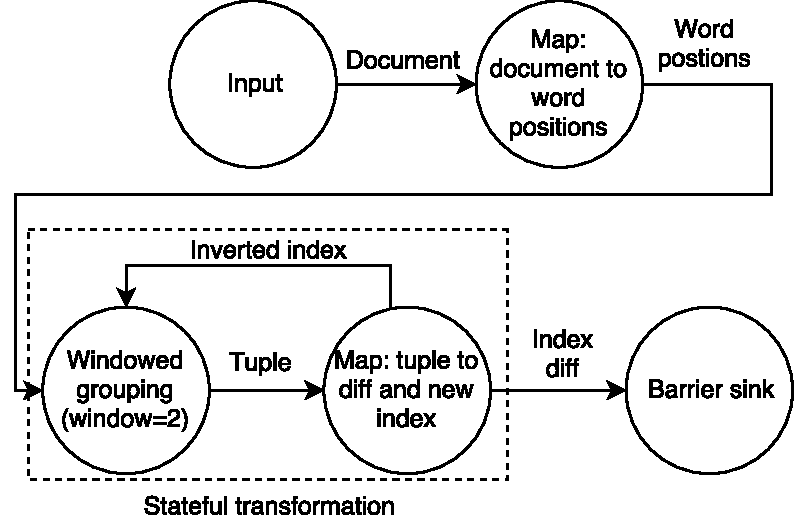
\includegraphics[width=0.48\textwidth]{pics/inverted-index}
  \caption{Logical pipeline for inverted index}
  \label {inverted-index}
\end{figure}

Our experiments were performed on clusters of 2, 4, 6, 8, and 10 nodes. Each node is an AWS EC2 micro instance with 1GB RAM and 1 core CPU.

As a key metric in our experiment, we take the ratio of arrived at the barrier items count to the number of the valid items among them. This value clearly represents the overhead of our approach, as it was mentioned at the end of the previous section. 

The relation between the number of workers, the delay between input documents and the proposed ratio is shown in Figure ~\ref{experiment}. As expected, the peak of the ratio is achieved when the document per second rate is high (greater than x rps) and the number of the nodes is low. This behaviour can be explained by the fact that a few workers cannot effectively deal with such intensive load. Nevertheless, the proportion of invalid items reduces with the increase of workers number. Under non-extreme load, the total overhead of the optimistic approach is under 10\% for all considered number of workers. These results confirm that the ratio does not increase with the growth of the number of nodes.

Therefore, the most important conclusions of the experiments are: the proposed method is scalable, the overhead could be optimized by system setup.

%% TODO: 
\begin{figure}[htbp]
  \centering
  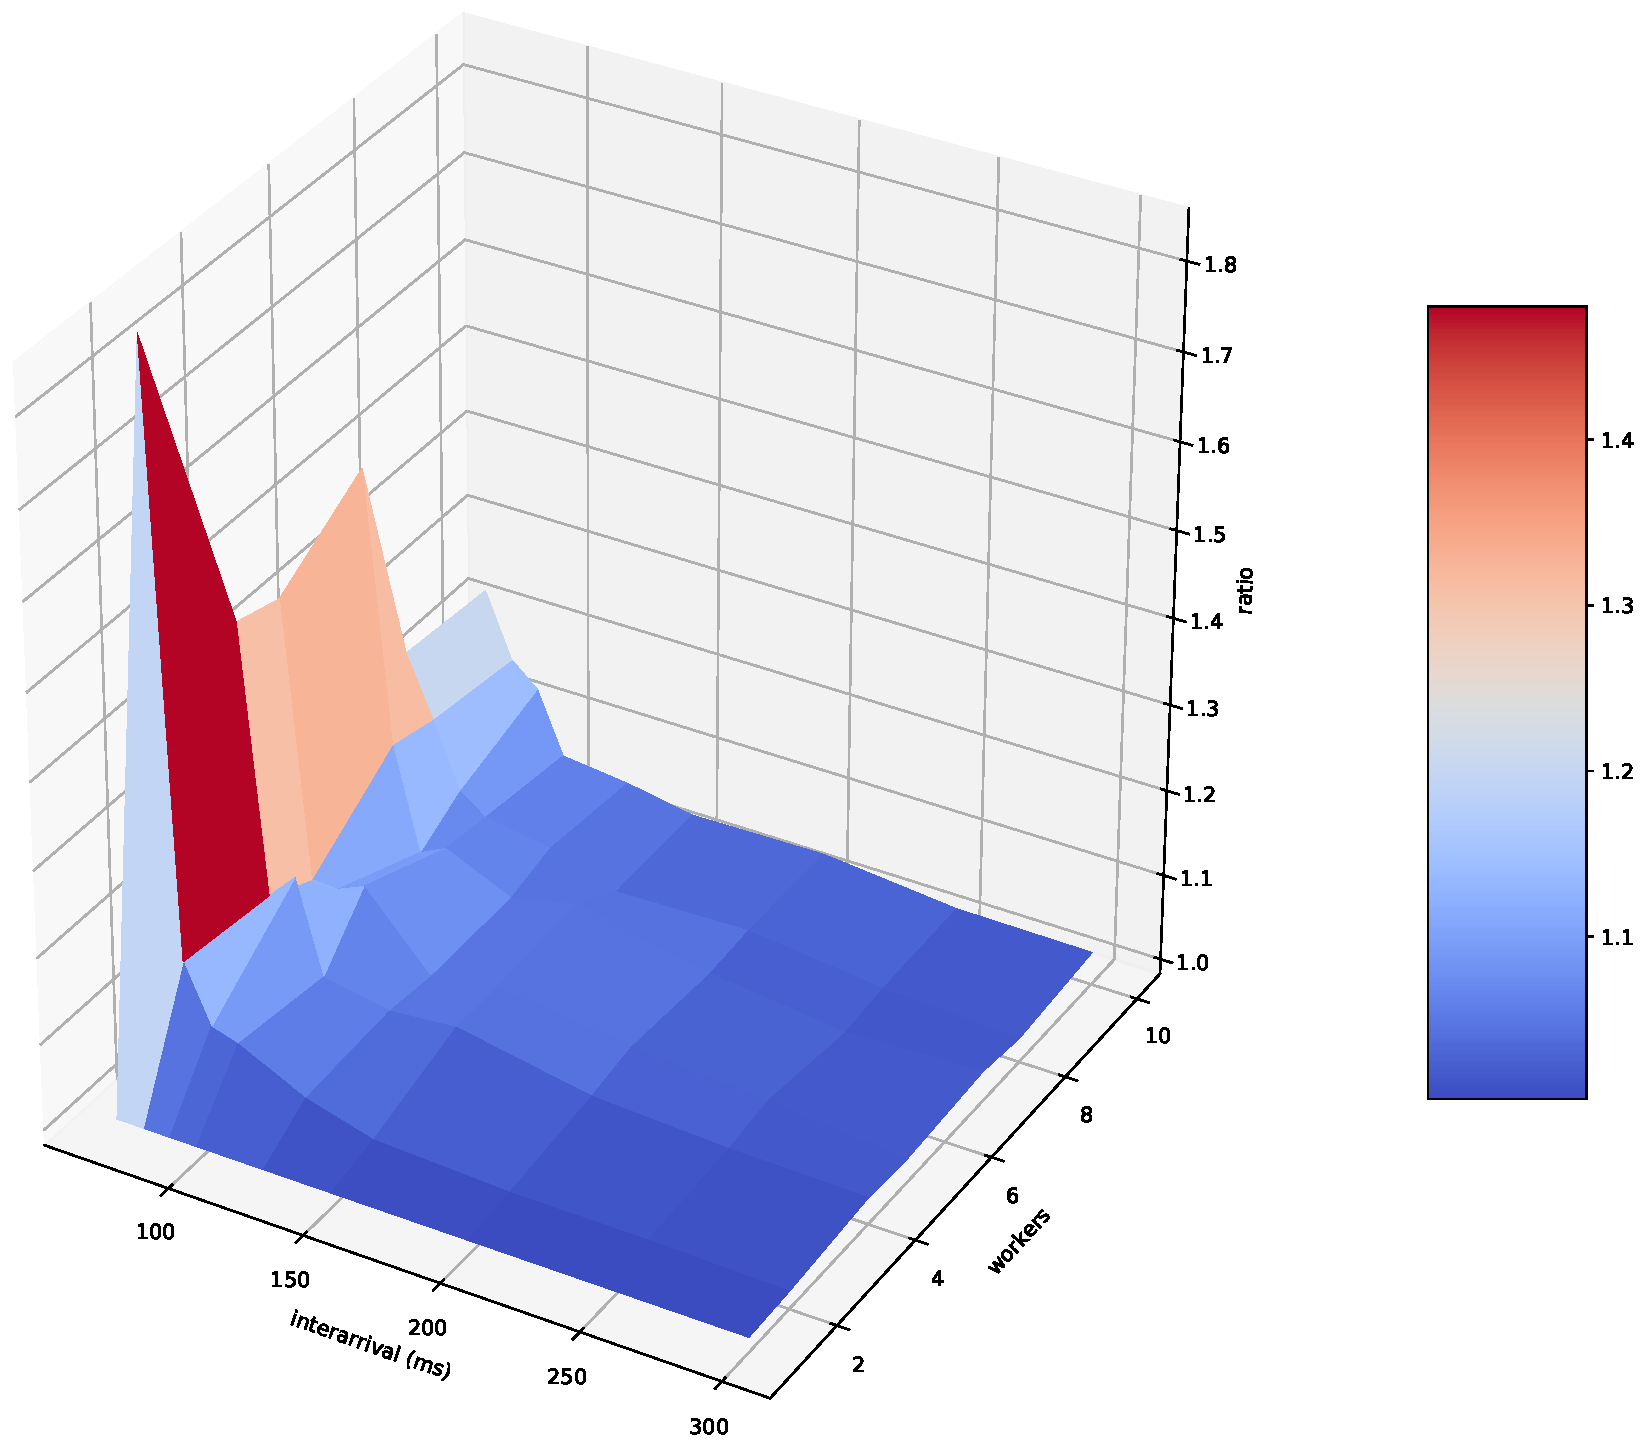
\includegraphics[width=0.48\textwidth]{pics/experiment}
  \caption{Experiment results}
  \label {experiment}
\end{figure}
